\documentclass[border=5pt]{standalone}
\usepackage{tikz}
\usepackage{amsmath,amssymb}
\usetikzlibrary{positioning, arrows.meta, calc, shapes.geometric}

% 颜色定义 - 参考 deep-direct-stat 风格
\definecolor{inputcolor}{RGB}{180, 130, 180}
\definecolor{convblue}{RGB}{70, 130, 180}
\definecolor{convdarkblue}{RGB}{50, 100, 150}
\definecolor{poolgreen}{RGB}{100, 160, 100}
\definecolor{fcgreen}{RGB}{140, 180, 100}
\definecolor{outputorange}{RGB}{220, 140, 80}
\definecolor{outputred}{RGB}{200, 100, 100}
\definecolor{outputyellow}{RGB}{220, 200, 100}
\definecolor{softmaxpurple}{RGB}{160, 100, 160}

\begin{document}
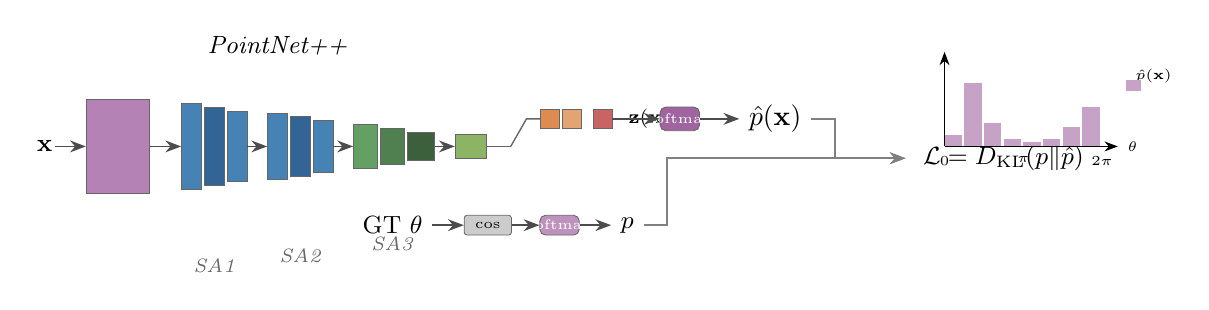
\begin{tikzpicture}[
    >=Stealth,
    layer/.style={minimum height=0.5cm, draw=black!60, line width=0.3pt},
    arrow/.style={->, line width=0.6pt, black!70},
    label/.style={font=\scriptsize},
]

% ===== 输入 =====
\node[layer, fill=inputcolor, minimum width=0.8cm, minimum height=1.2cm] (input) at (0,0) {};
\node[left=0.3cm of input, font=\small] {$\mathbf{x}$};
\draw[arrow] (-0.8,0) -- (input.west);

% ===== PointNet++ Backbone =====
% SA1
\node[layer, fill=convblue, minimum width=0.25cm, minimum height=1.1cm, right=0.4cm of input] (sa1a) {};
\node[layer, fill=convdarkblue, minimum width=0.25cm, minimum height=1.0cm, right=0.03cm of sa1a] (sa1b) {};
\node[layer, fill=convblue, minimum width=0.25cm, minimum height=0.9cm, right=0.03cm of sa1b] (sa1c) {};

% SA2
\node[layer, fill=convblue, minimum width=0.25cm, minimum height=0.85cm, right=0.25cm of sa1c] (sa2a) {};
\node[layer, fill=convdarkblue, minimum width=0.25cm, minimum height=0.75cm, right=0.03cm of sa2a] (sa2b) {};
\node[layer, fill=convblue, minimum width=0.25cm, minimum height=0.65cm, right=0.03cm of sa2b] (sa2c) {};

% SA3 (Global)
\node[layer, fill=poolgreen, minimum width=0.3cm, minimum height=0.55cm, right=0.25cm of sa2c] (sa3a) {};
\node[layer, fill=poolgreen!80!black, minimum width=0.3cm, minimum height=0.45cm, right=0.03cm of sa3a] (sa3b) {};
\node[layer, fill=poolgreen!60!black, minimum width=0.35cm, minimum height=0.35cm, right=0.03cm of sa3b] (sa3c) {};

% 全局特征
\node[layer, fill=fcgreen, minimum width=0.4cm, minimum height=0.3cm, right=0.25cm of sa3c] (global) {};

% 箭头
\draw[arrow] (input.east) -- (sa1a.west);
\draw[arrow] (sa1c.east) -- (sa2a.west);
\draw[arrow] (sa2c.east) -- (sa3a.west);
\draw[arrow] (sa3c.east) -- (global.west);

% Backbone 标签
\node[above=0.6cm of sa2a, font=\small\itshape] {PointNet++};

% ===== Classification Head - 多分支输出 =====
\coordinate (branch) at ($(global.east)+(0.3,0)$);

% 上分支: logits
\node[layer, fill=outputorange, minimum width=0.15cm, minimum height=0.25cm] (fc1) at ($(branch)+(0.5, 0.35)$) {};
\node[layer, fill=outputorange!80, minimum width=0.15cm, minimum height=0.2cm, right=0.03cm of fc1] (fc2) {};
\node[layer, fill=outputred, minimum width=0.12cm, minimum height=0.15cm, right=0.15cm of fc2] (logits) {};

% 分支线
\draw[line width=0.5pt, black!60] (global.east) -- (branch);
\draw[line width=0.5pt, black!60] (branch) -- ($(branch)+(0.2, 0.35)$) -- (fc1.west);

% logits 标签
\node[right=0.08cm of logits, font=\scriptsize] {$\mathbf{z}(\mathbf{x})$};

% ===== Softmax =====
\node[layer, fill=softmaxpurple, minimum width=0.5cm, minimum height=0.3cm, rounded corners=2pt, right=0.6cm of logits] (softmax) {};
\node[font=\tiny, text=white] at (softmax) {softmax};

\draw[arrow] (logits.east) -- (softmax.west);

% ===== 预测分布 =====
\node[right=0.5cm of softmax] (predprob) {$\hat{p}(\mathbf{x})$};
\draw[arrow] (softmax.east) -- (predprob.west);

% ===== GT 分支 (下方) =====
% GT 输入
\node[font=\small] (gtlabel) at ($(branch)+(-1.5, -1.0)$) {GT $\theta$};

% cos projection
\node[layer, fill=black!20, minimum width=0.6cm, minimum height=0.25cm, rounded corners=1pt, right=0.4cm of gtlabel] (cosproj) {};
\node[font=\tiny] at (cosproj) {$\cos$};

% GT softmax
\node[layer, fill=softmaxpurple!70, minimum width=0.5cm, minimum height=0.25cm, rounded corners=2pt, right=0.35cm of cosproj] (gtsoftmax) {};
\node[font=\tiny, text=white] at (gtsoftmax) {softmax};

% GT prob
\node[right=0.4cm of gtsoftmax, font=\small] (gtprob) {$p$};

\draw[arrow] (gtlabel.east) -- (cosproj.west);
\draw[arrow] (cosproj.east) -- (gtsoftmax.west);
\draw[arrow] (gtsoftmax.east) -- (gtprob.west);

% ===== Loss =====
\coordinate (losscenter) at ($(predprob.east)+(1.2, -0.5)$);

% 箭头到 loss
\draw[arrow, black!50] (predprob.east) -- ++(0.3,0) |- (losscenter);
\draw[arrow, black!50] (gtprob.east) -- ++(0.3,0) |- (losscenter);

% Loss 公式
\node[right=0.1cm of losscenter, font=\small] {$\mathcal{L} = D_{\mathrm{KL}}(p \| \hat{p})$};

% ===== 分布可视化 (右侧) =====
\begin{scope}[shift={(10.5, 0)}]
    % 坐标轴
    \draw[->] (0,0) -- (2.2,0) node[right, font=\tiny] {$\theta$};
    \draw[->] (0,0) -- (0,1.2);

    % 刻度
    \node[below, font=\tiny] at (0,0) {$0$};
    \node[below, font=\tiny] at (1,0) {$\pi$};
    \node[below, font=\tiny] at (2,0) {$2\pi$};

    % 预测分布 (8 bins 柱状图)
    \foreach \i/\h in {0/0.15, 1/0.8, 2/0.3, 3/0.1, 4/0.05, 5/0.1, 6/0.25, 7/0.5} {
        \fill[softmaxpurple!60] (\i*0.25, 0) rectangle (\i*0.25+0.22, \h);
    }

    % 图例
    \node[font=\tiny, right] at (2.3, 0.9) {$\hat{p}(\mathbf{x})$};
    \fill[softmaxpurple!60] (2.3, 0.7) rectangle (2.5, 0.85);
\end{scope}

% ===== 底部标注 =====
\node[below=0.8cm of sa1b, font=\scriptsize\itshape, text=black!60] {SA1};
\node[below=0.8cm of sa2b, font=\scriptsize\itshape, text=black!60] {SA2};
\node[below=0.8cm of sa3b, font=\scriptsize\itshape, text=black!60] {SA3};

\end{tikzpicture}
\end{document}
